\renewcommand\thesection{\Alph{section}}
\renewcommand\thesubsection{\thesection.\arabic{subsection}}
\setcounter{section}{1}
\section{Entrega acumulada B}

\setcounter{subsection}{1}
\subsection{Se deben implementar al menos 3 ventanas gráficas (GUIs en AWTo SWING): 1 ventana de menú, 1 ventana de agregar elemento y 1 ventana de listar elementos}

Cuando inicializa el programa puede emerger una ventana en caso de una correcta conexión con la base de datos o de caso contrario un error y la opcion de trabajar con datos locales.

\begin{multicols}{2}
    \successBox{Conexión correcta}{
        \centering
        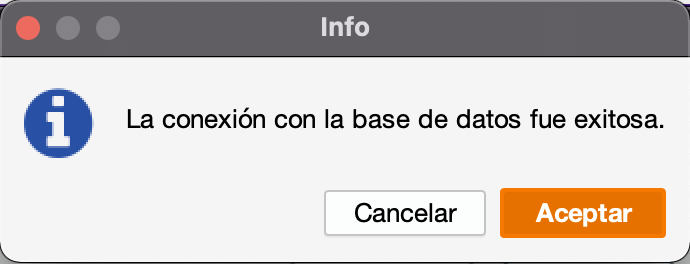
\includegraphics[width=0.7\textwidth]{contents/img/gui/img20}
        \label{fig:gui20}
        \vspace{8.5mm}
        \\Se utilizan los datos de la base de datos.
        \vspace{8.5mm}
    }

    \columnbreak

    \warningBox{Conexión no realizada}{
        \centering
        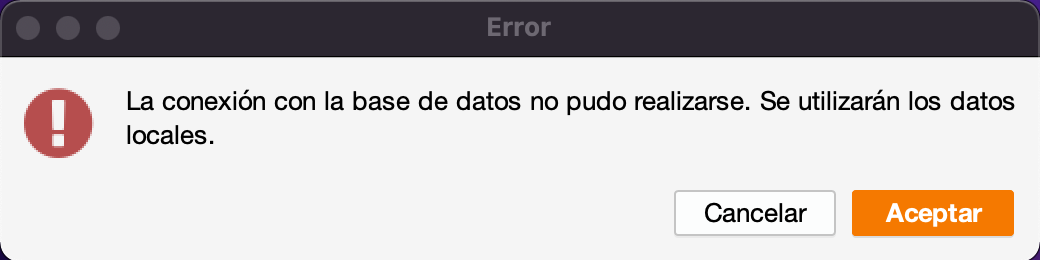
\includegraphics[width=1\textwidth]{contents/img/gui/img1}
        \label{fig:gui1}
        \\No se pudo realizar la conexión a la base de datos. Se utilizarán los datos locales en su lugar, que corresponden a los archivos CSV ubicados en la carpeta \textbf{datafiles}, ubicada en la raiz del proyecto.
    }
\end{multicols}

A continuacion se muestra la ventana de bienvenida, al lado izquierdo se ve el menú que será visible en todo momento para navegar fácilmente cuando sea requerido dentro de las funcionalidades del programa.

\begin{figure}[h]
    \centering
    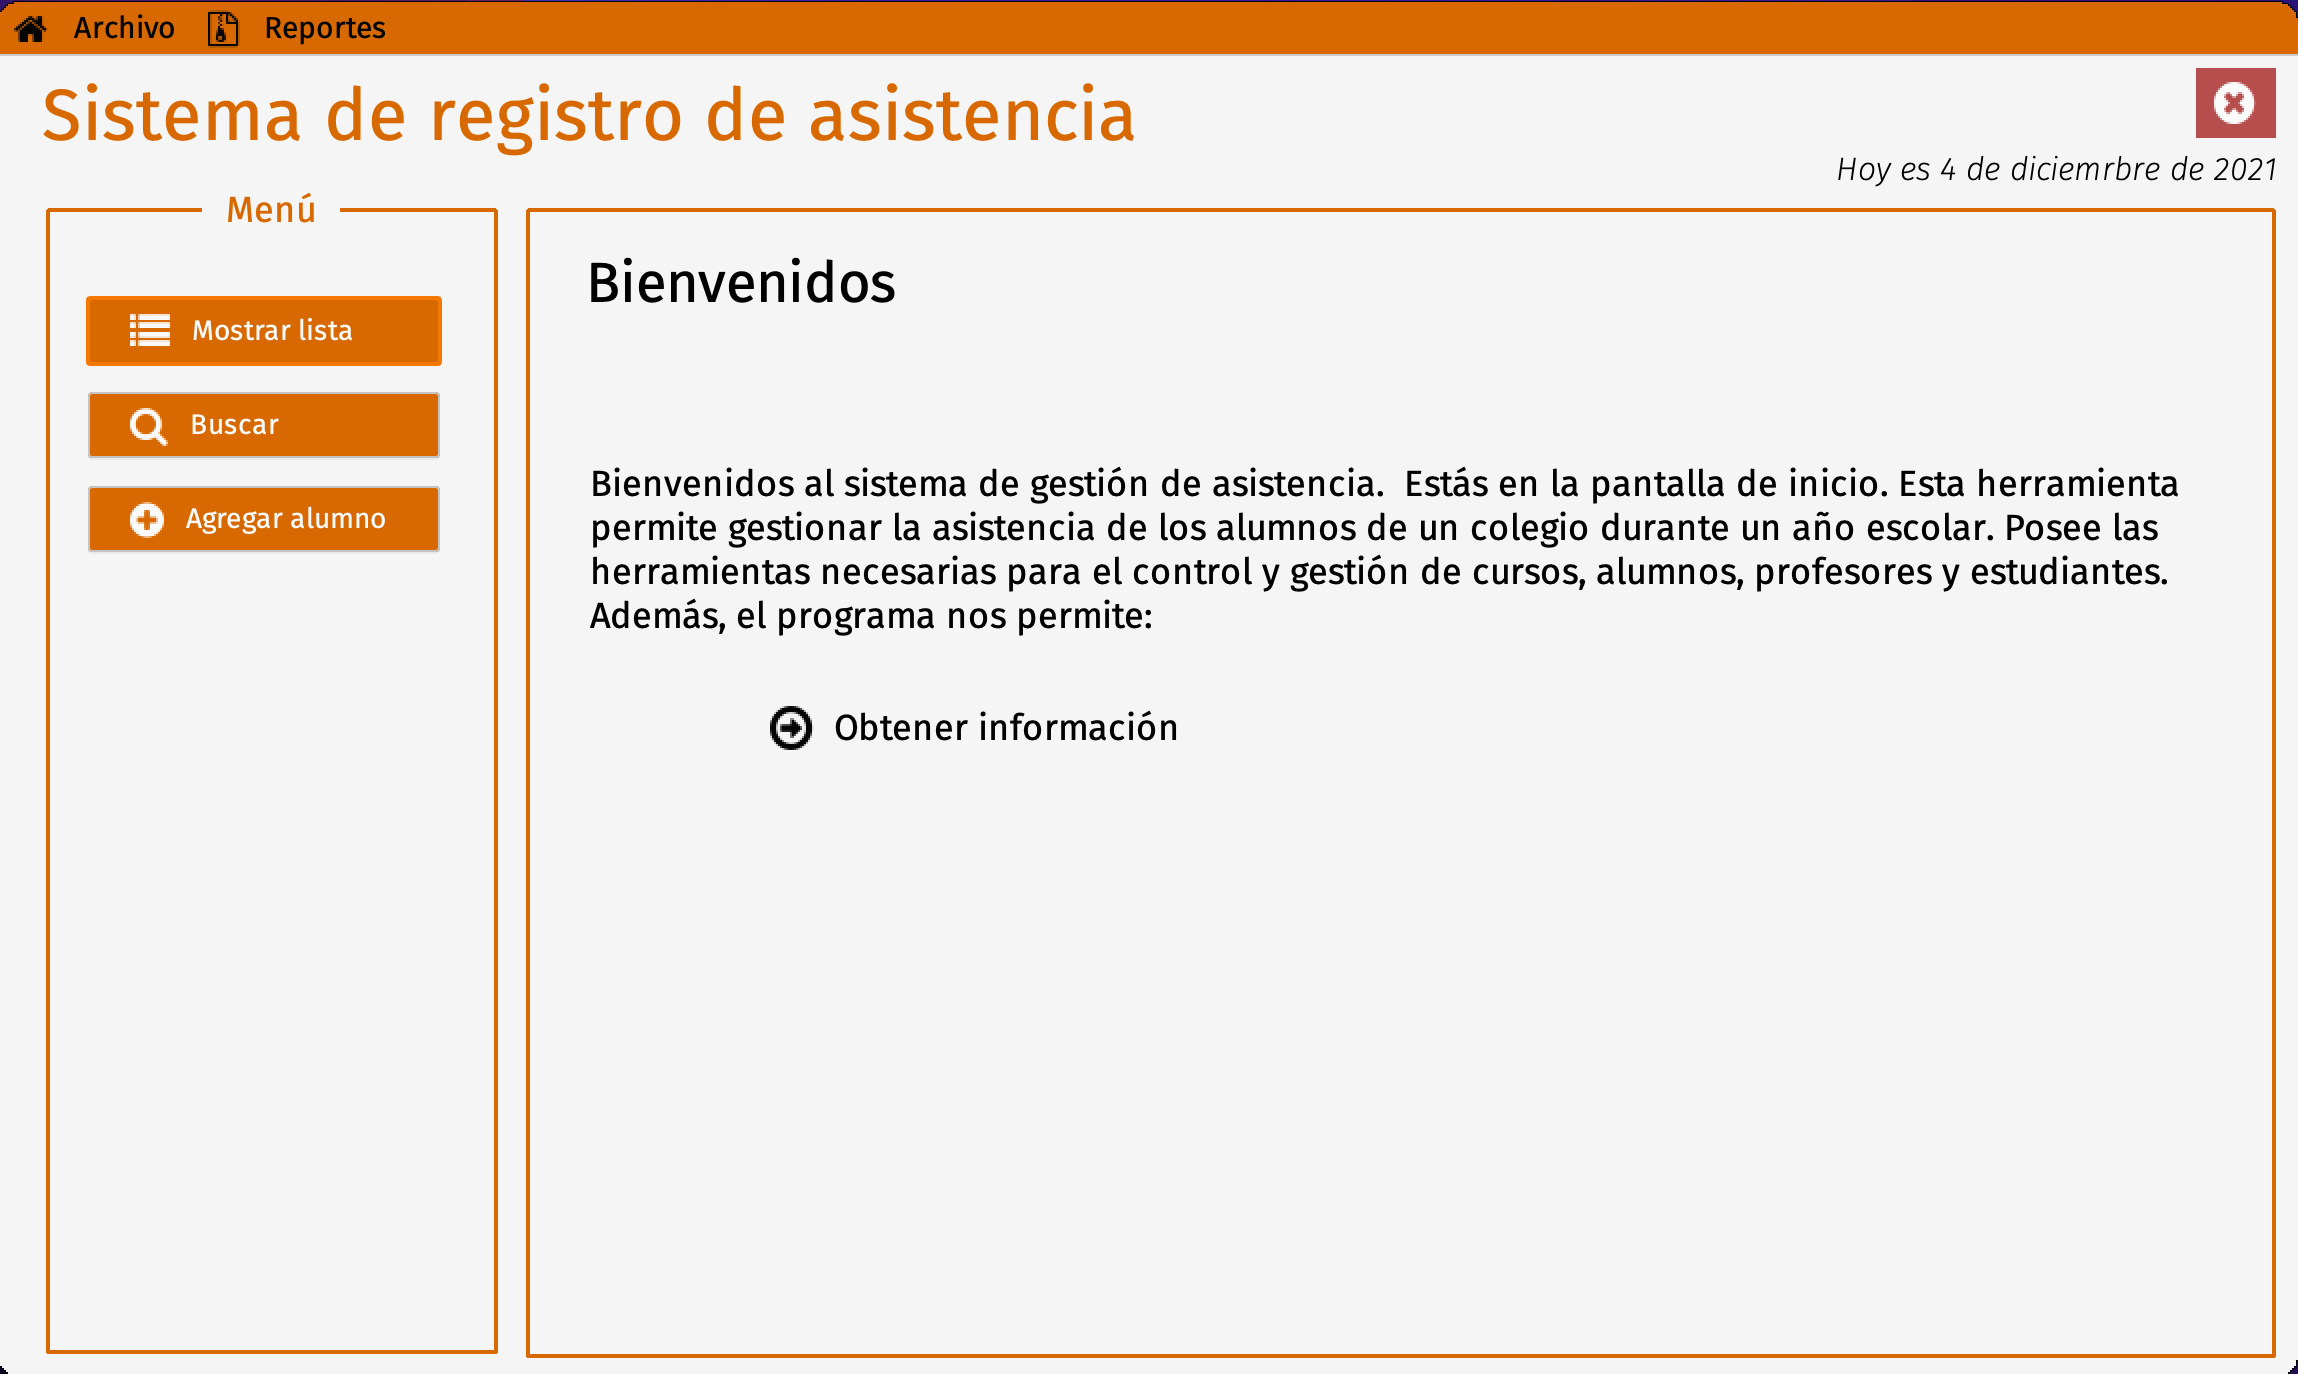
\includegraphics[width=0.9\textwidth]{contents/img/gui/img2}
    \caption{Ventana de bienvenida al programa}
    \label{fig:gui2}
\end{figure}

\subsubsection*{Extra: Modo oscuro}

Gracias a la inclusión de la librería externa \textbf{FlatLaf}, y su inclusión de diferentes estilos y colores gráficos para \textbf{Java Swing}, el programa puede cambiar su apariencia en tiempo de ejecución, lo que permite incorporar la opción de ver el programa en \textbf{modo oscuro}, opción de la que se puede acceder mediante el menú superior de la ventana.

\infoBox{Modo oscuro}{%
    \centering
    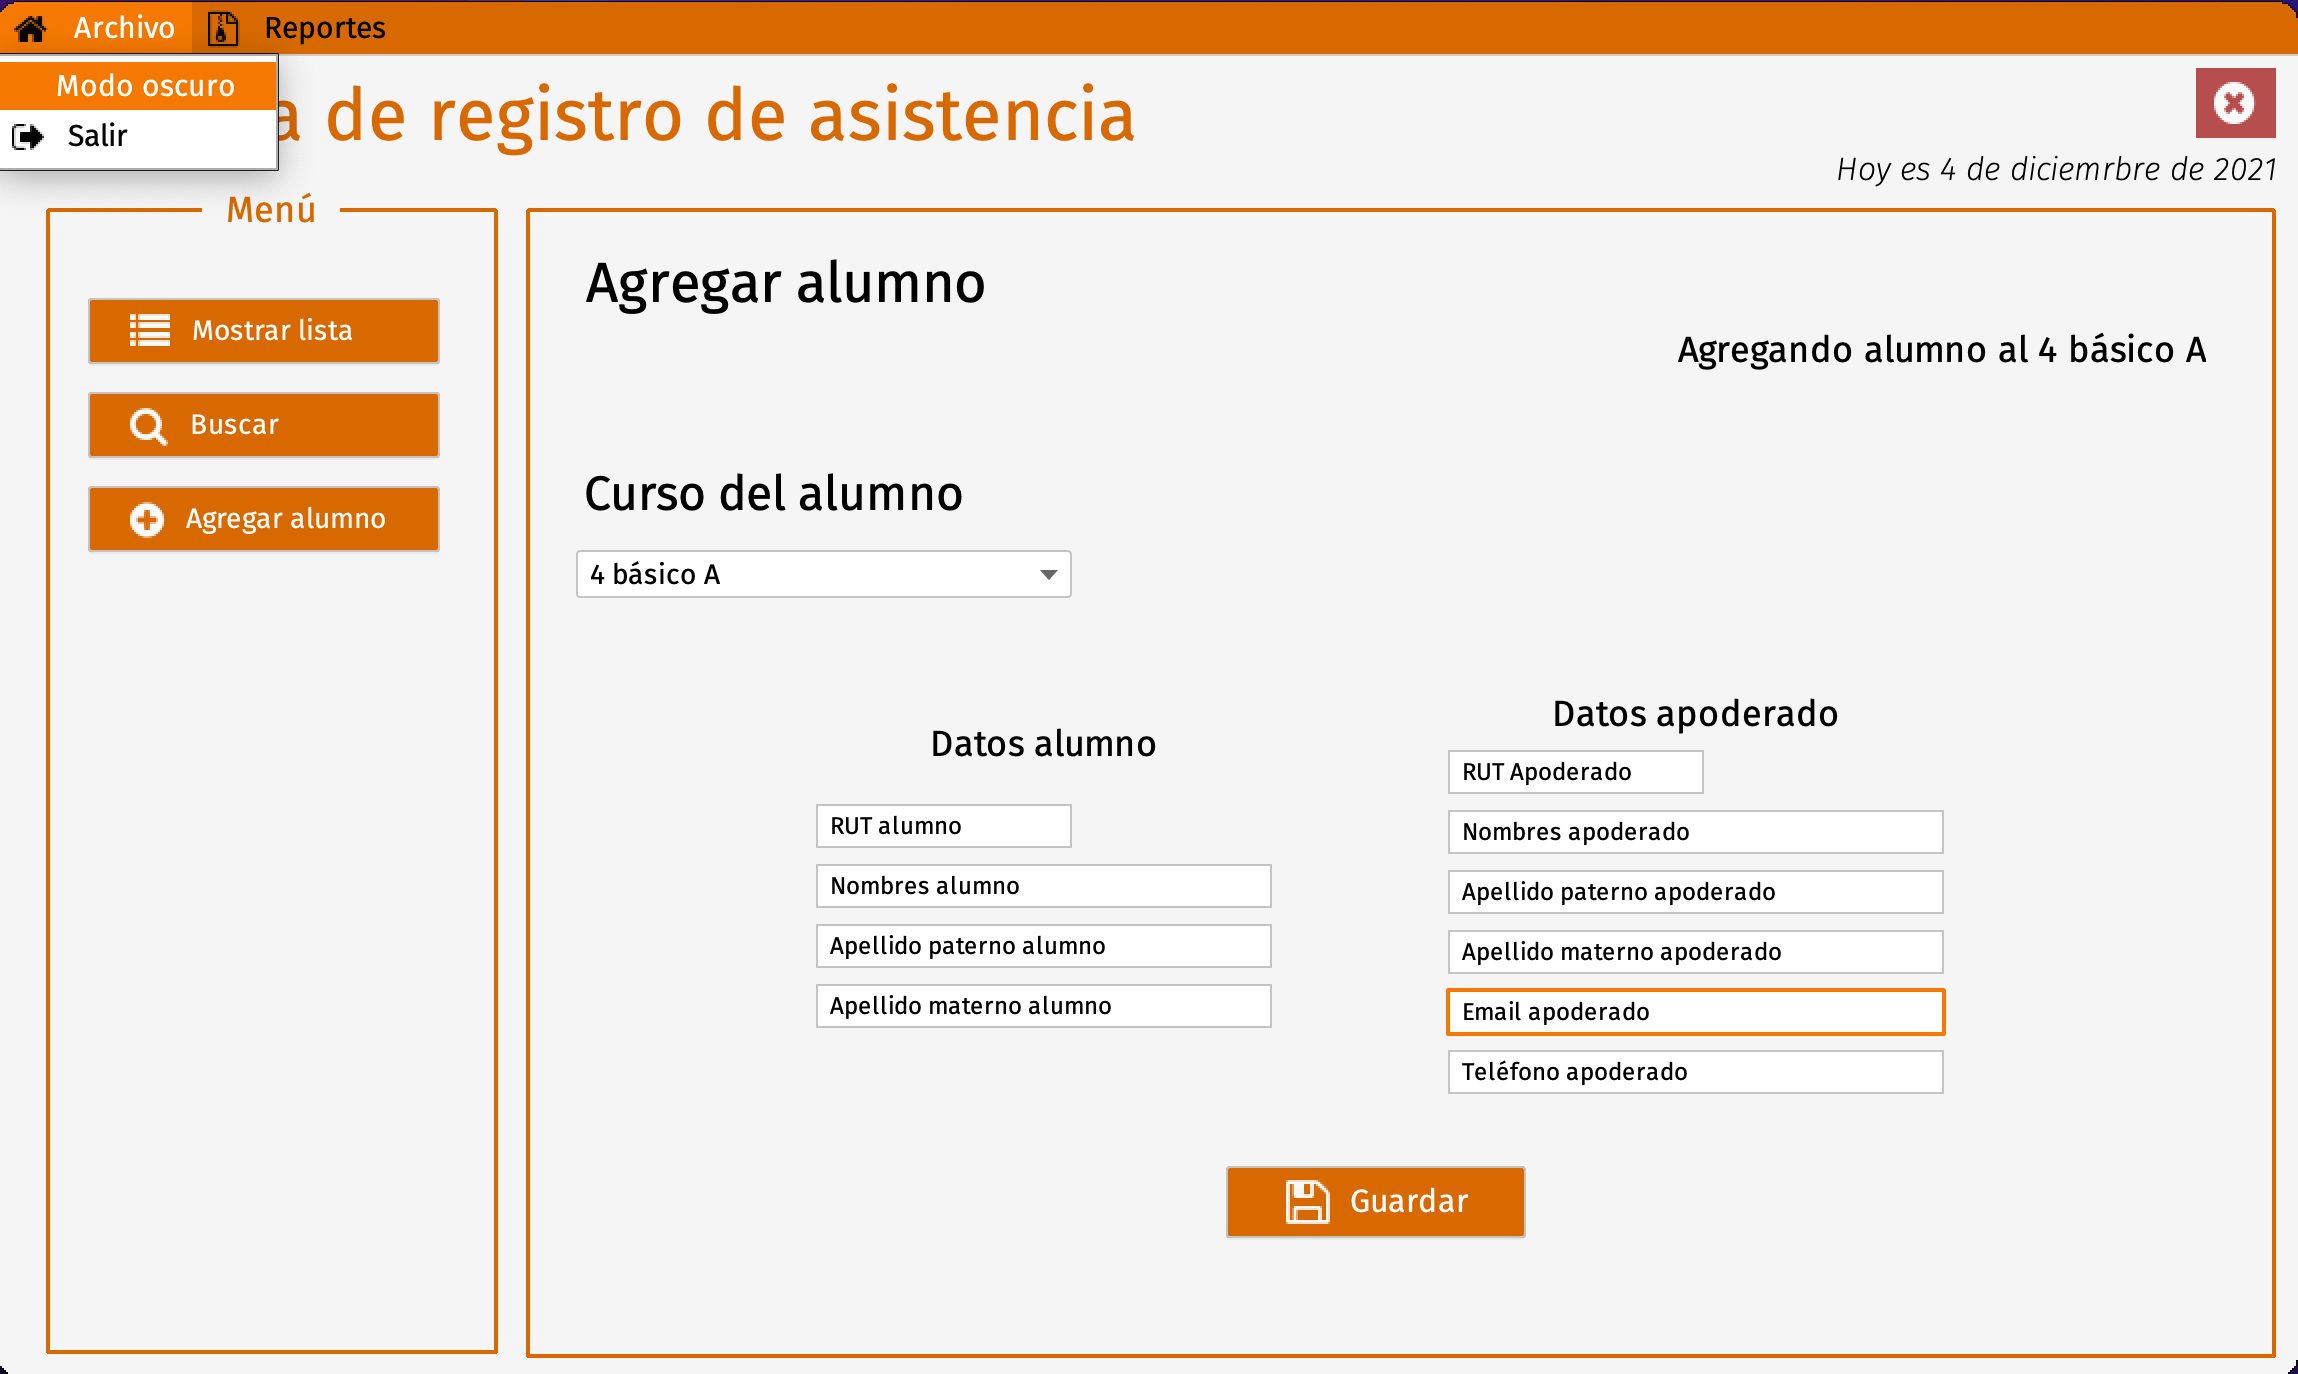
\includegraphics[width=1\textwidth]{contents/img/gui/img11}
    \label{fig:gui11}
    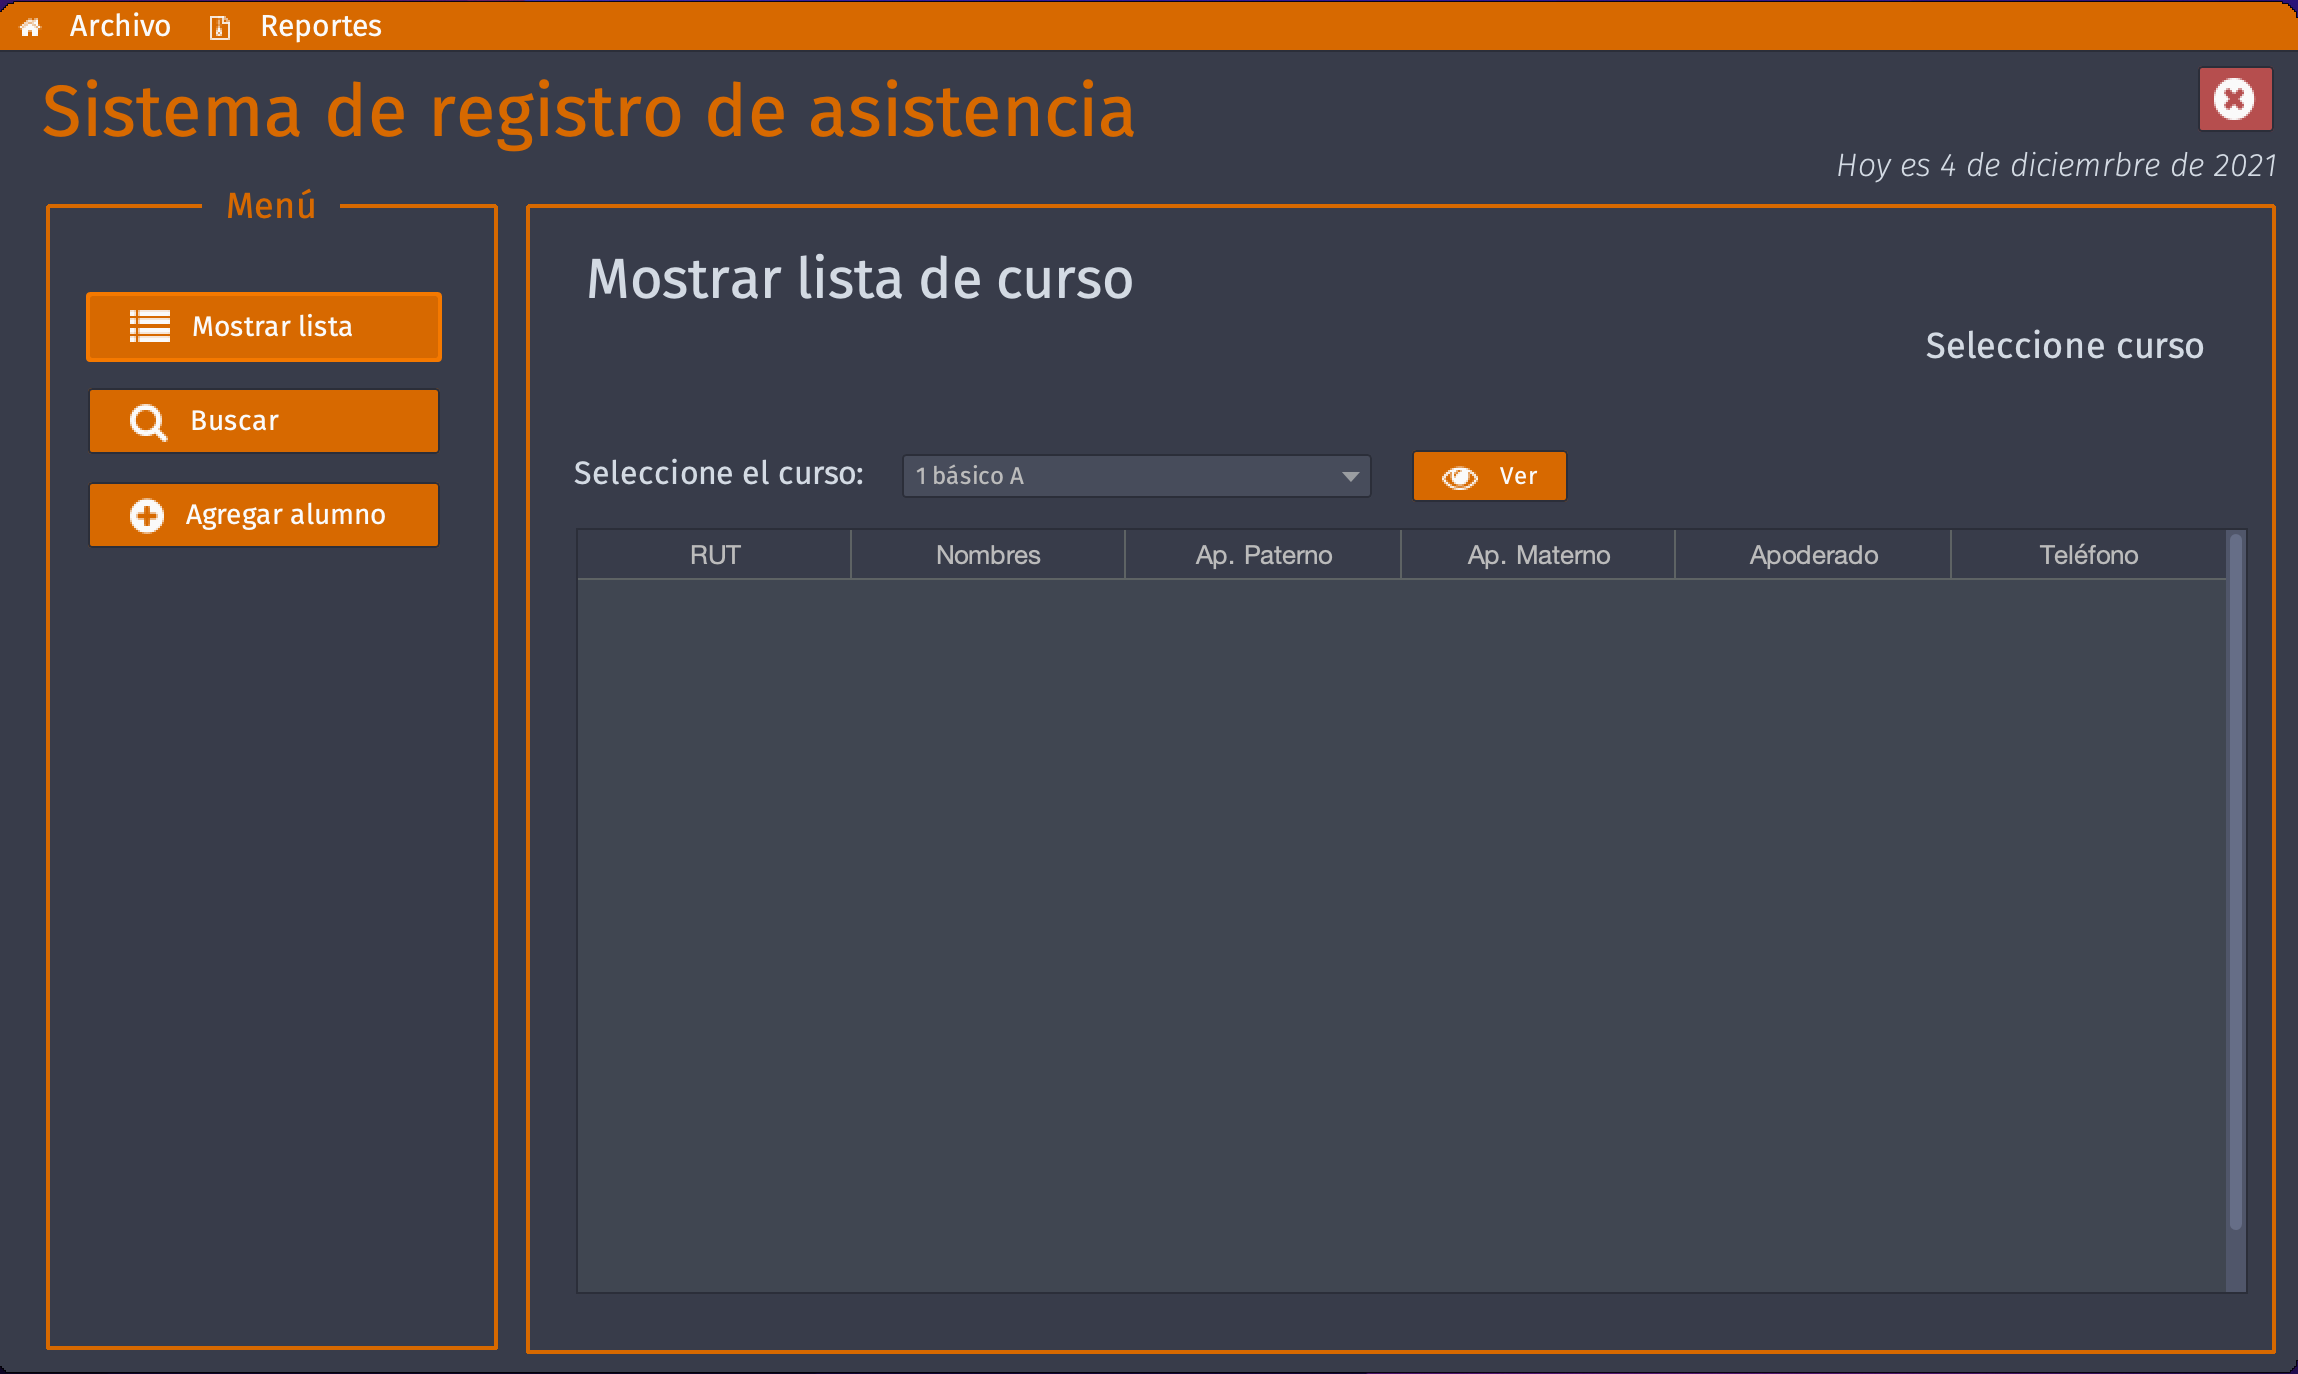
\includegraphics[width=1\textwidth]{contents/img/gui/img12}
    \label{fig:gui12}
}

La interfaz gráfica también nos permite las siguientes operaciones:

\textbf{Agregar un nuevo alumno}

\clearpage

\begin{figure}[h]
    \centering
    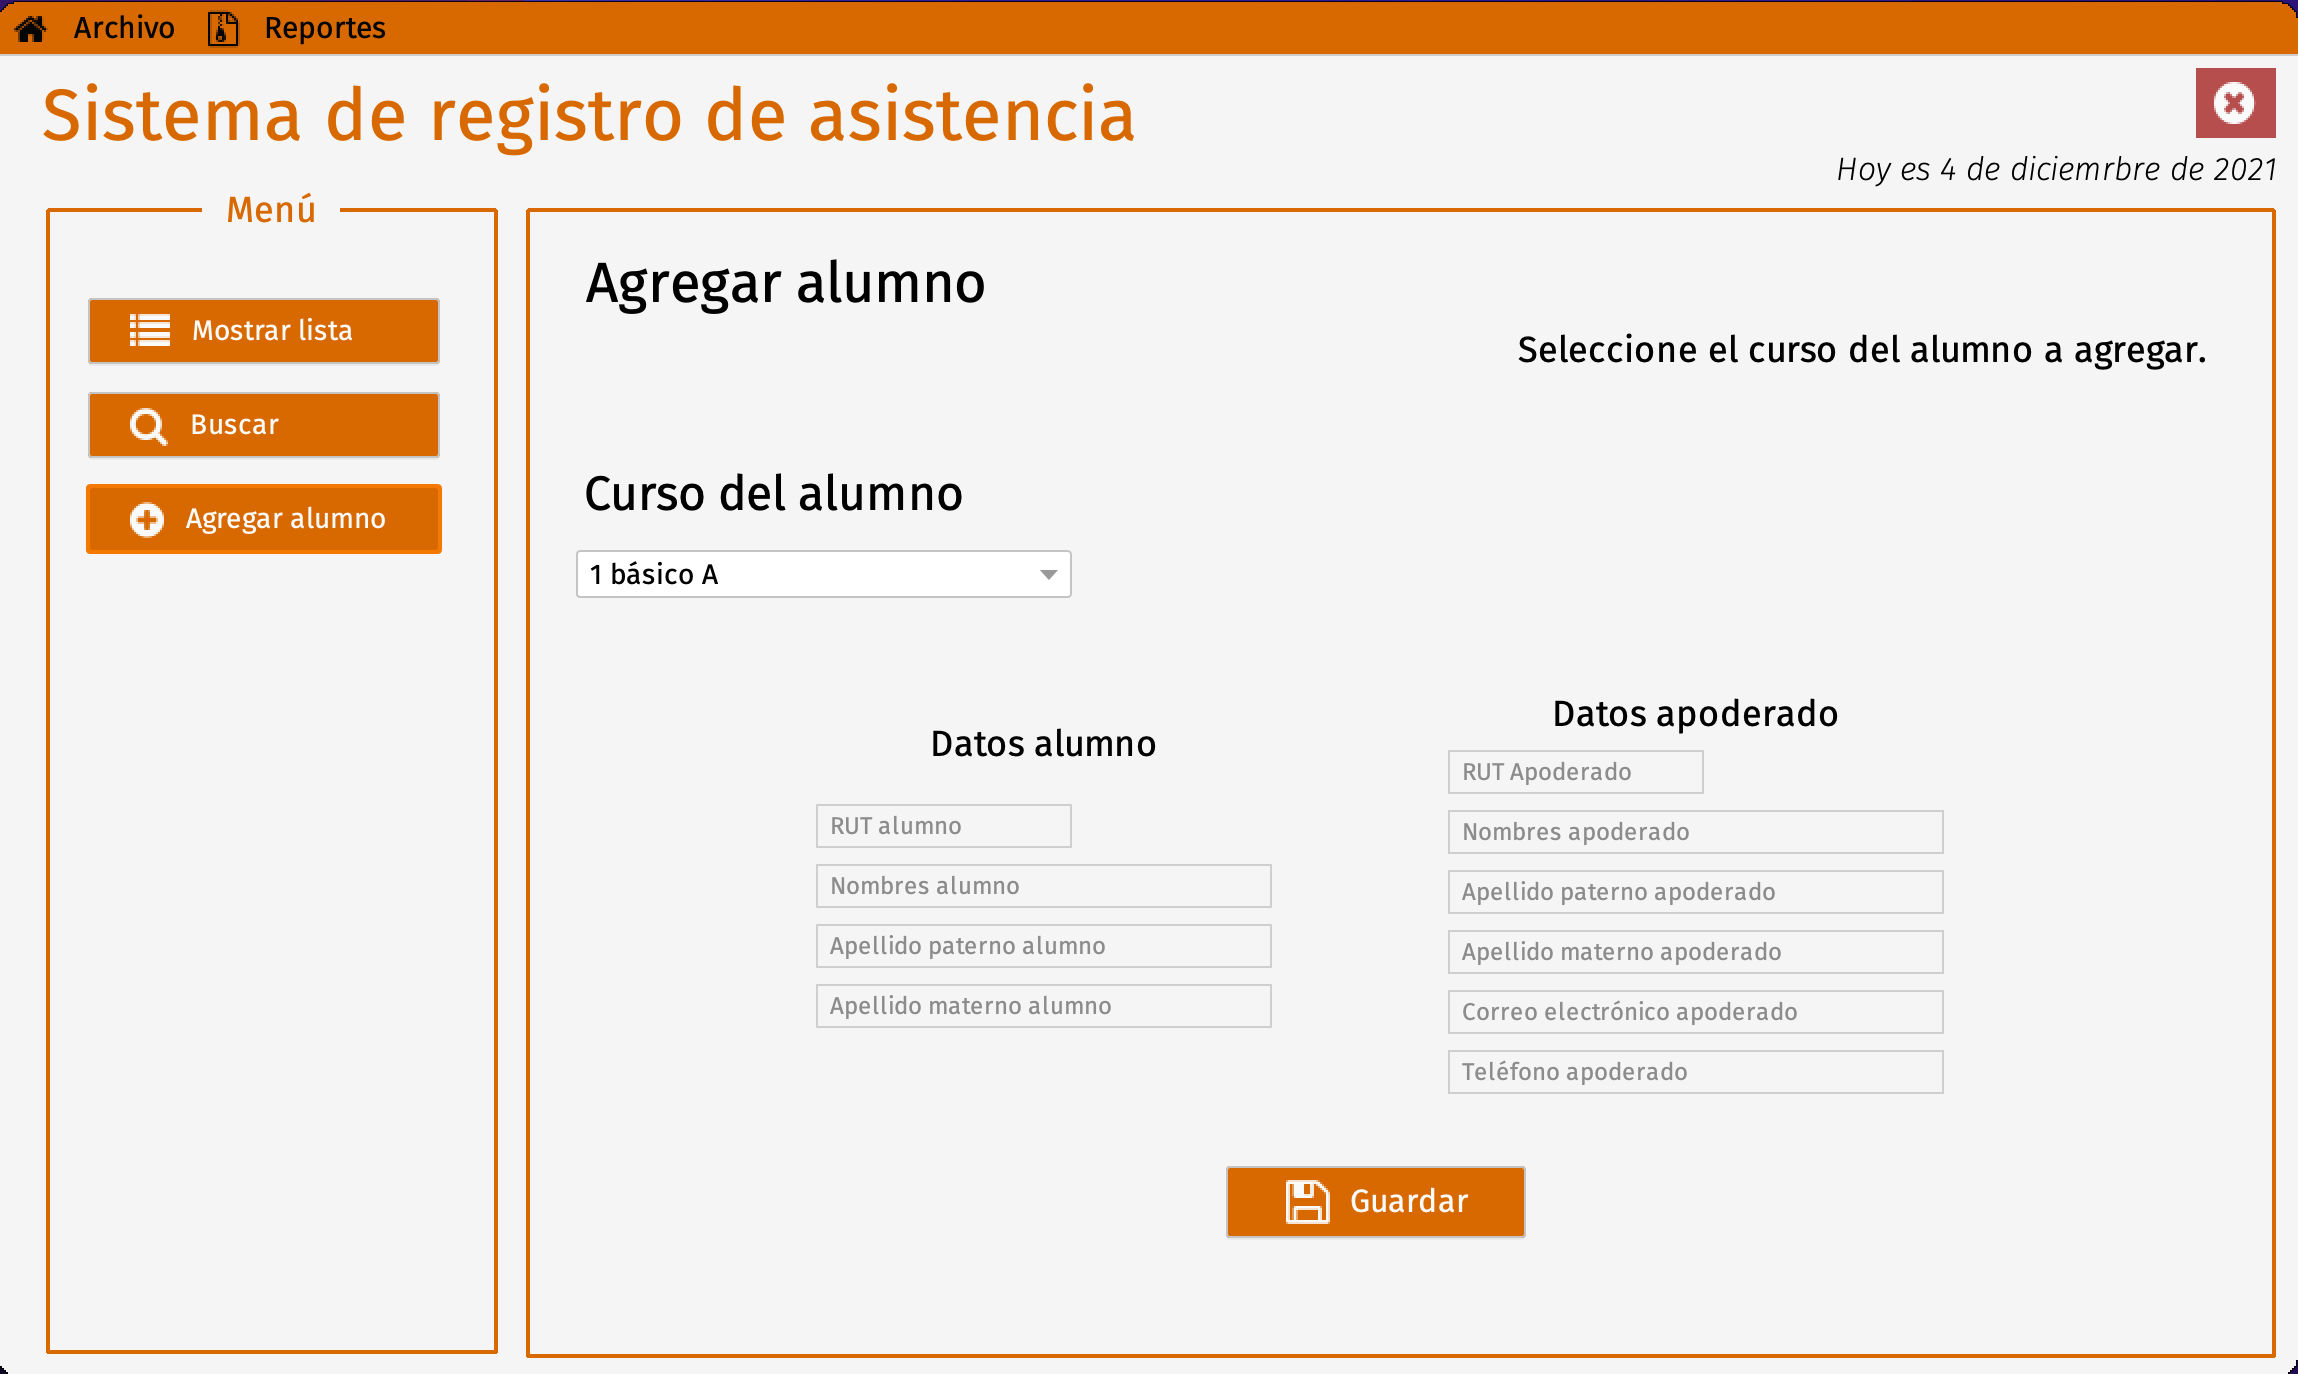
\includegraphics[width=0.9\textwidth]{contents/img/gui/img8}
    \caption{Ventana para agregar un nuevo alumno}
    \label{fig:gui8}
\end{figure}

\textbf{OJO:} La ventana posee un validador para el número de teléfono, aceptando sólo caracteres numéricos, y arrojando una excepción en caso de recibir cualquier otro caracter, mostrando una alerta al usuario.

\errorBox{Error al ingresar número de teléfono}{%
    \centering
    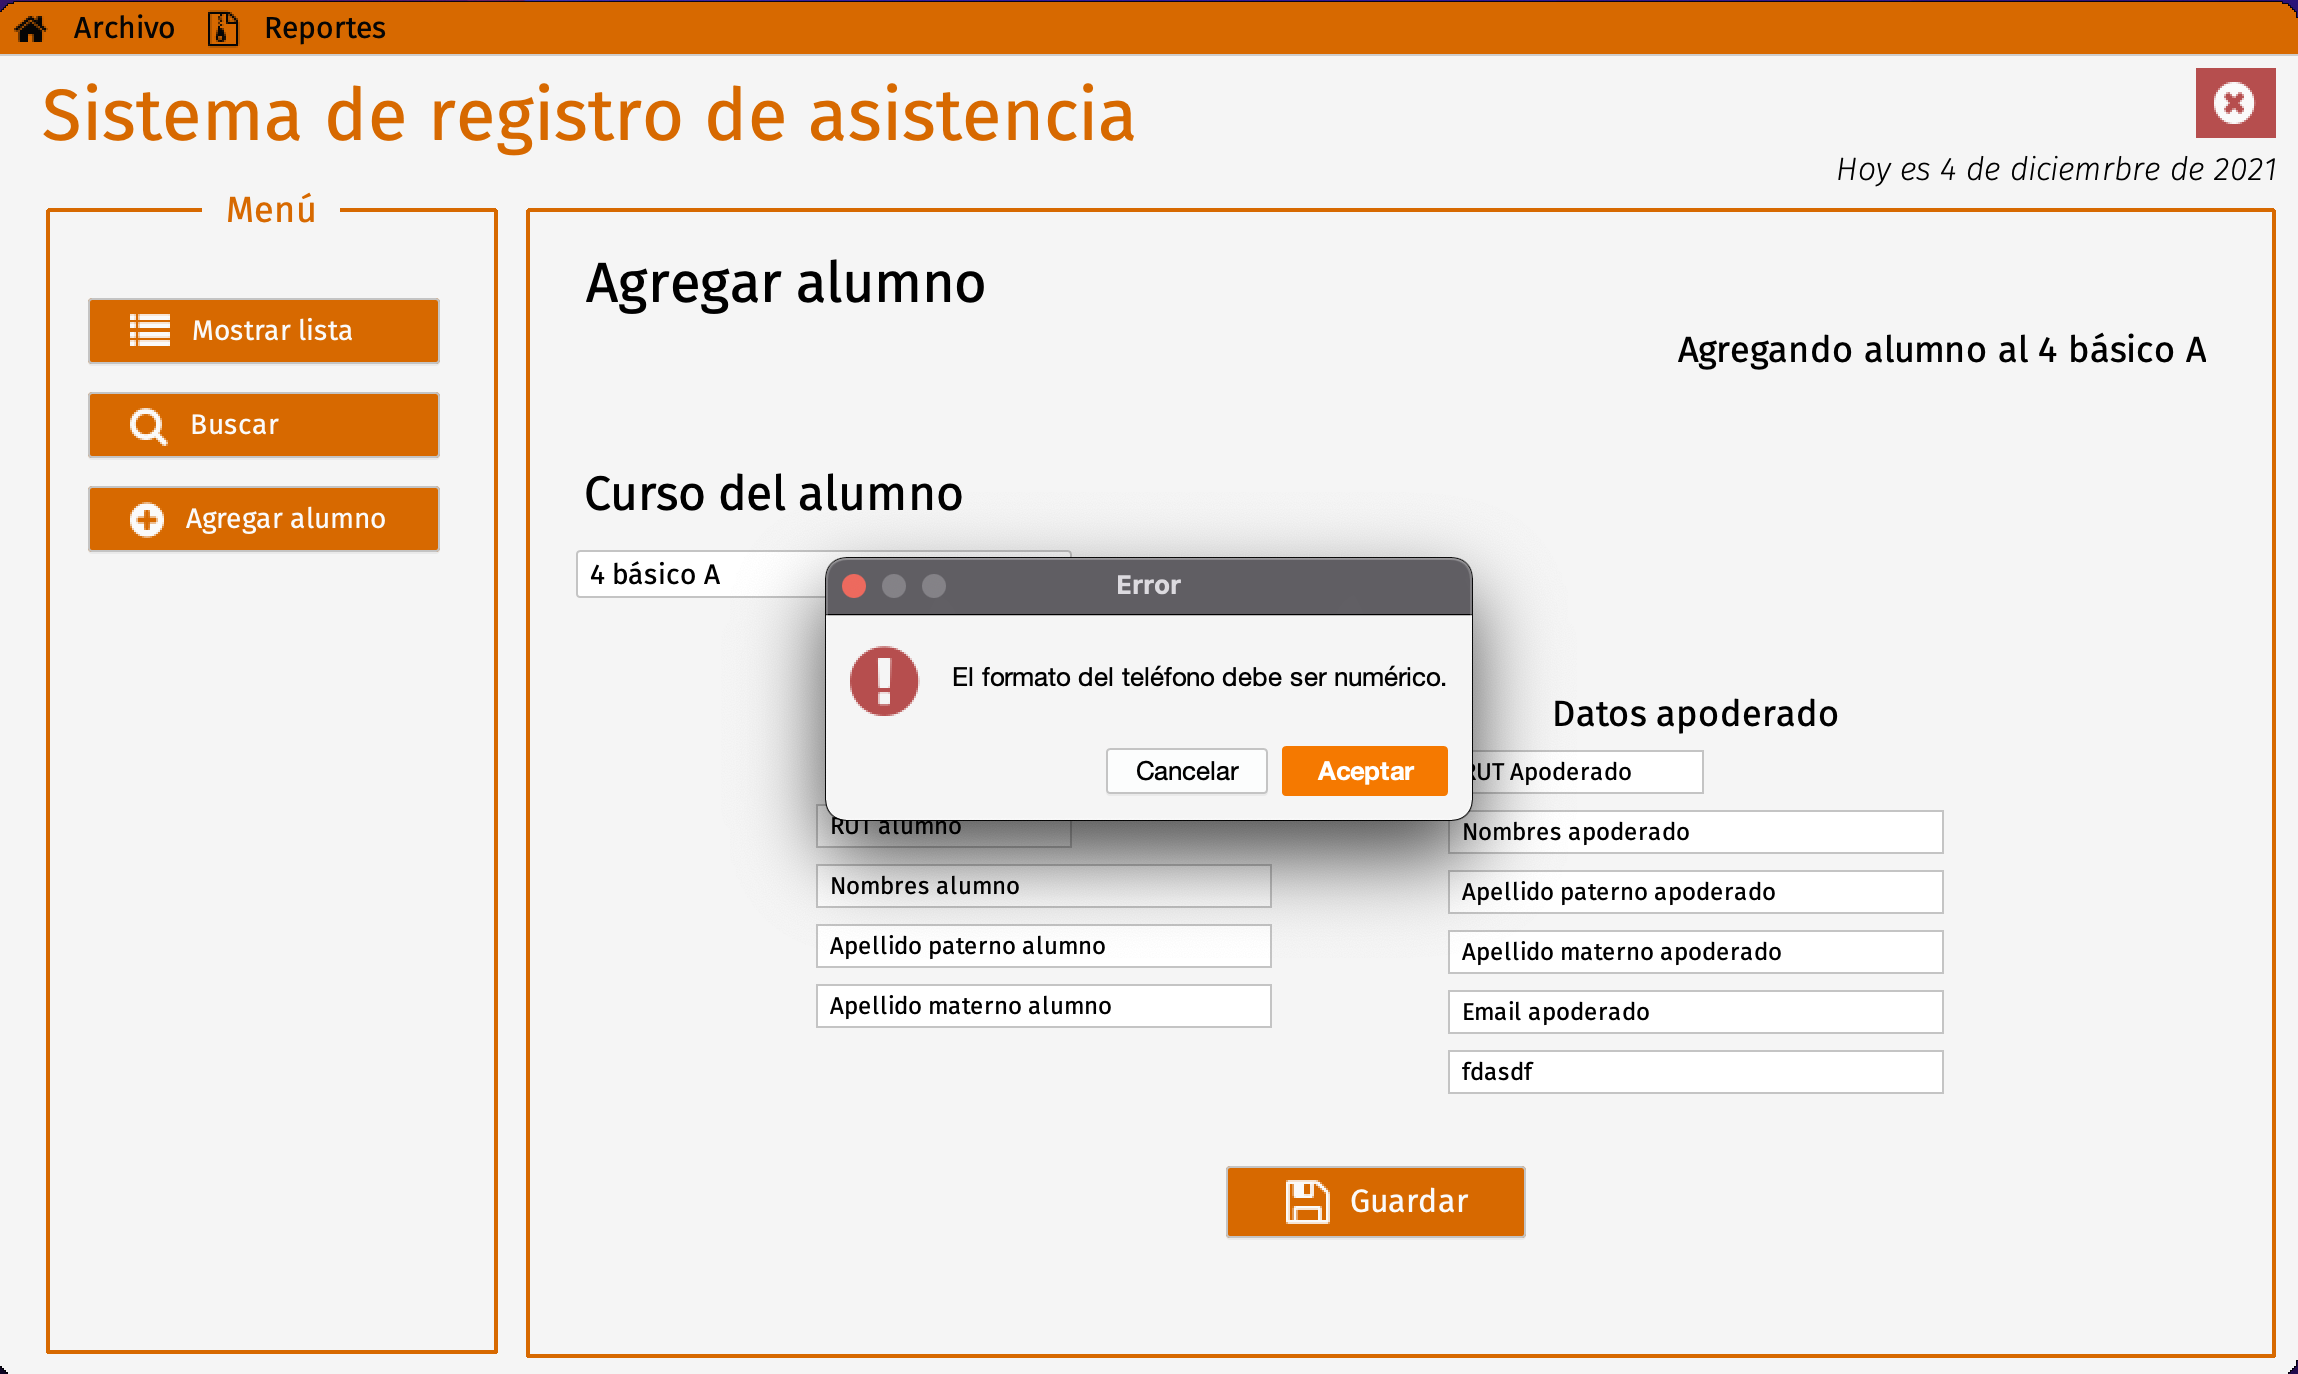
\includegraphics[width=1\textwidth]{contents/img/gui/img10}
    \label{fig:gui10}
}

\clearpage

\textbf{Listar cursos}

\begin{figure}[h]
    \centering
    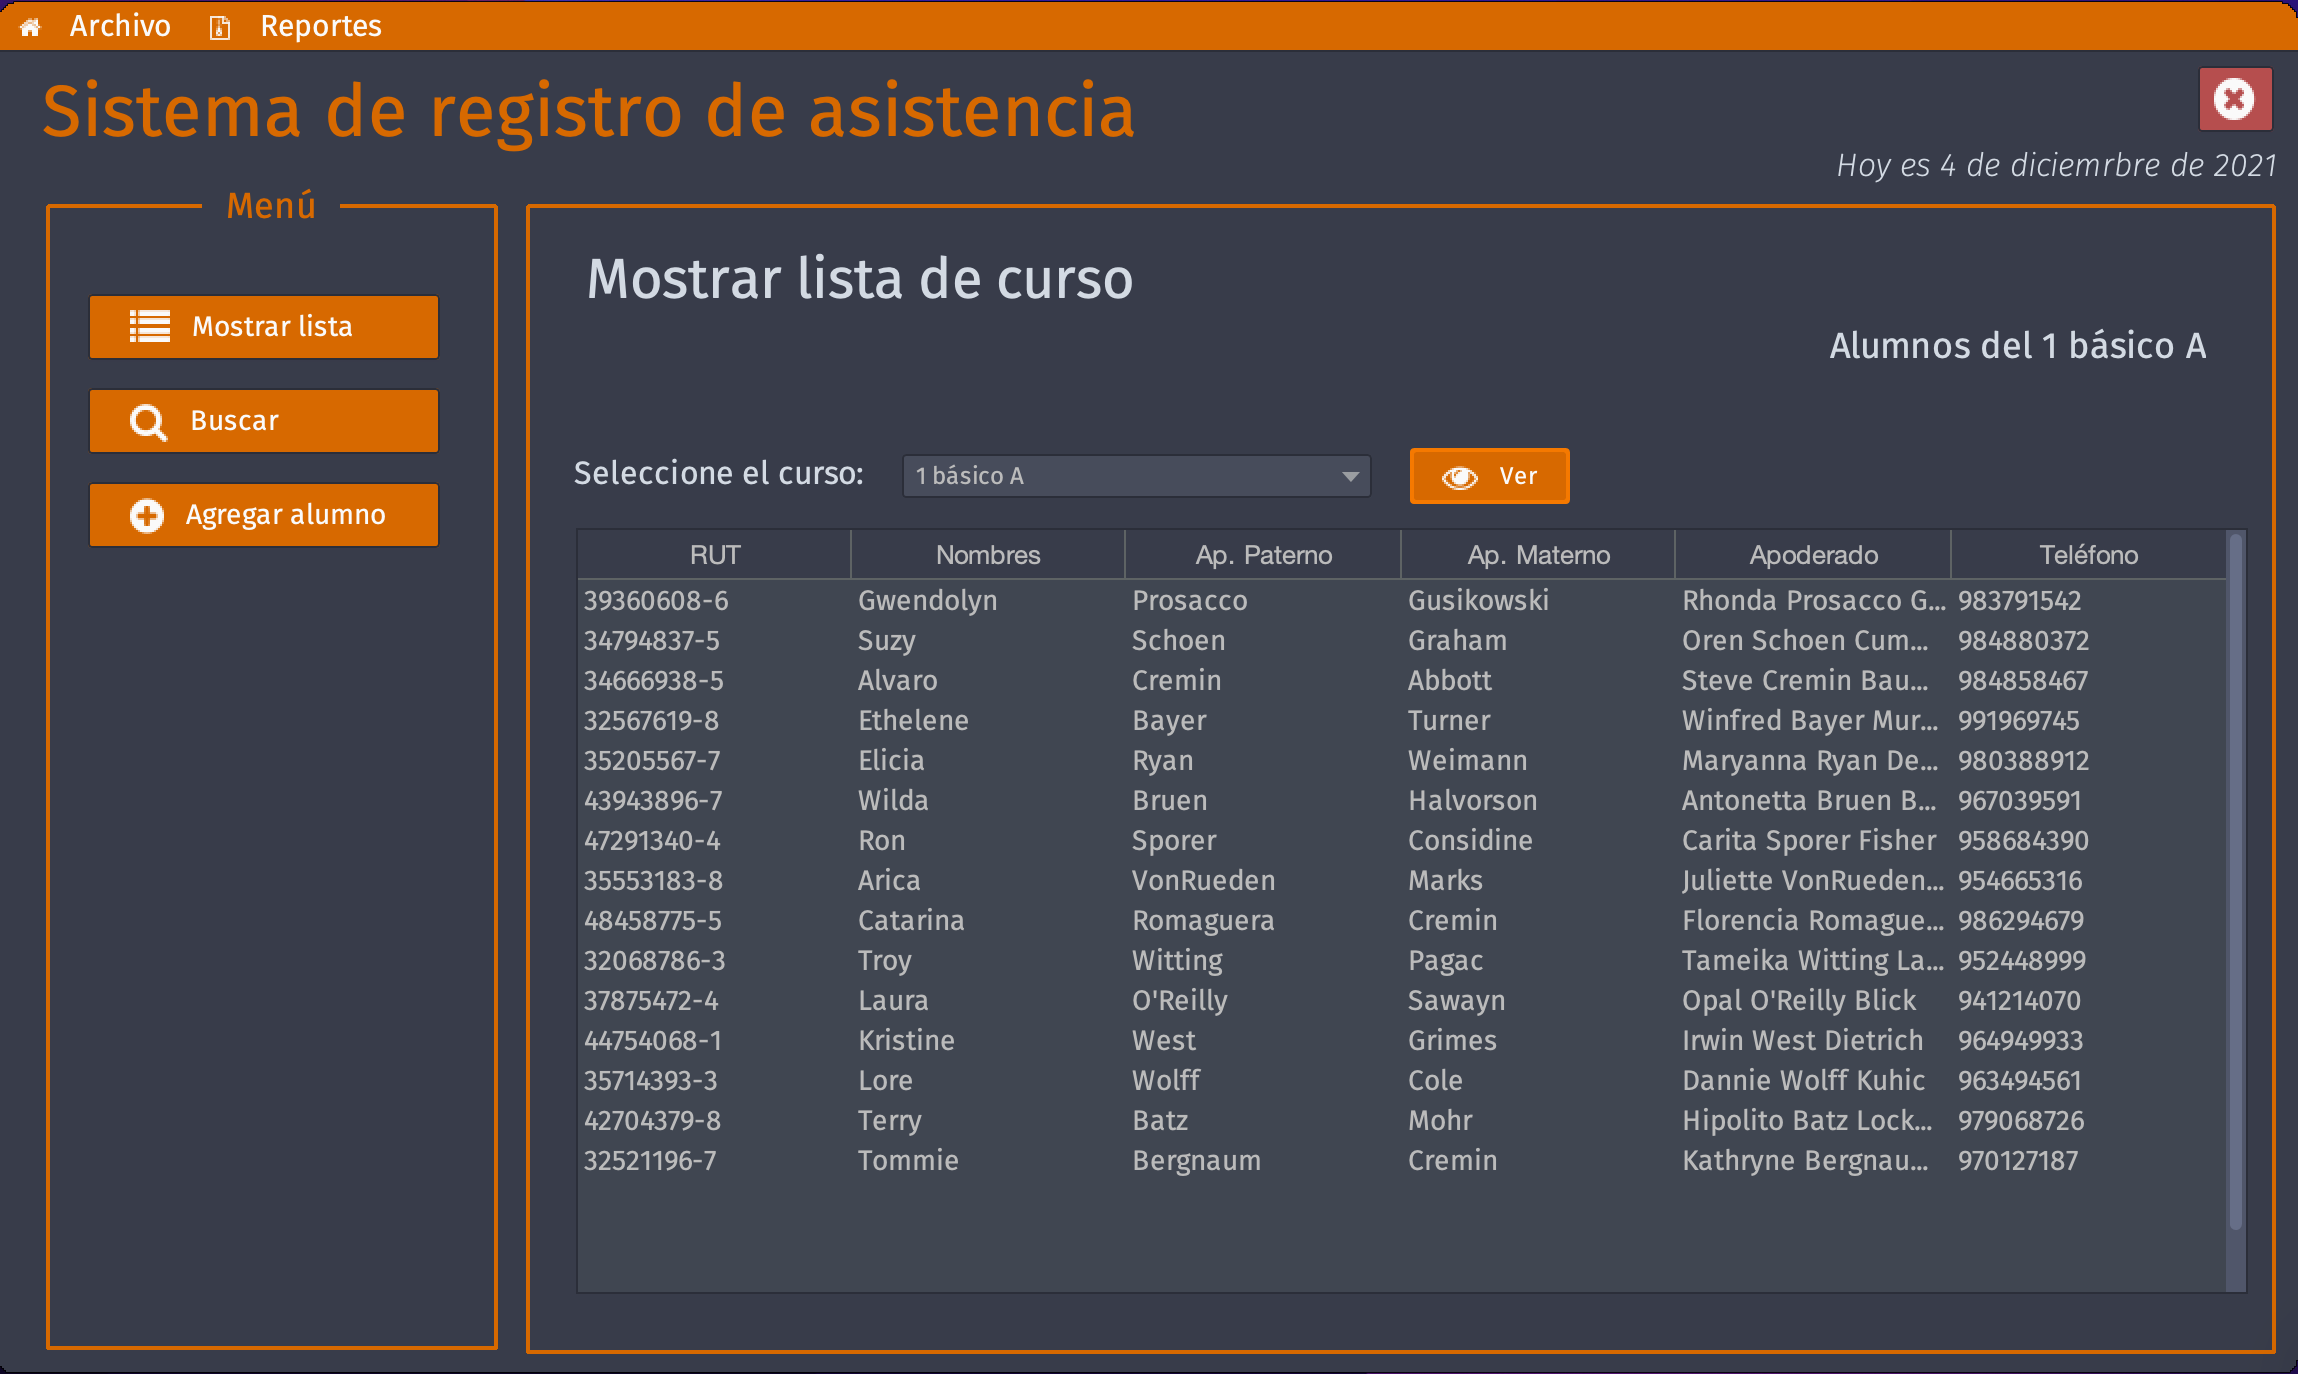
\includegraphics[width=0.7\textwidth]{contents/img/gui/img13}
    \caption{Ventana para mostrar lista de curso específico}
    \label{fig:gui13}
\end{figure}

\textbf{Buscar persona (alumno, profesor o apoderado)}

\begin{figure}[h]
    \centering
    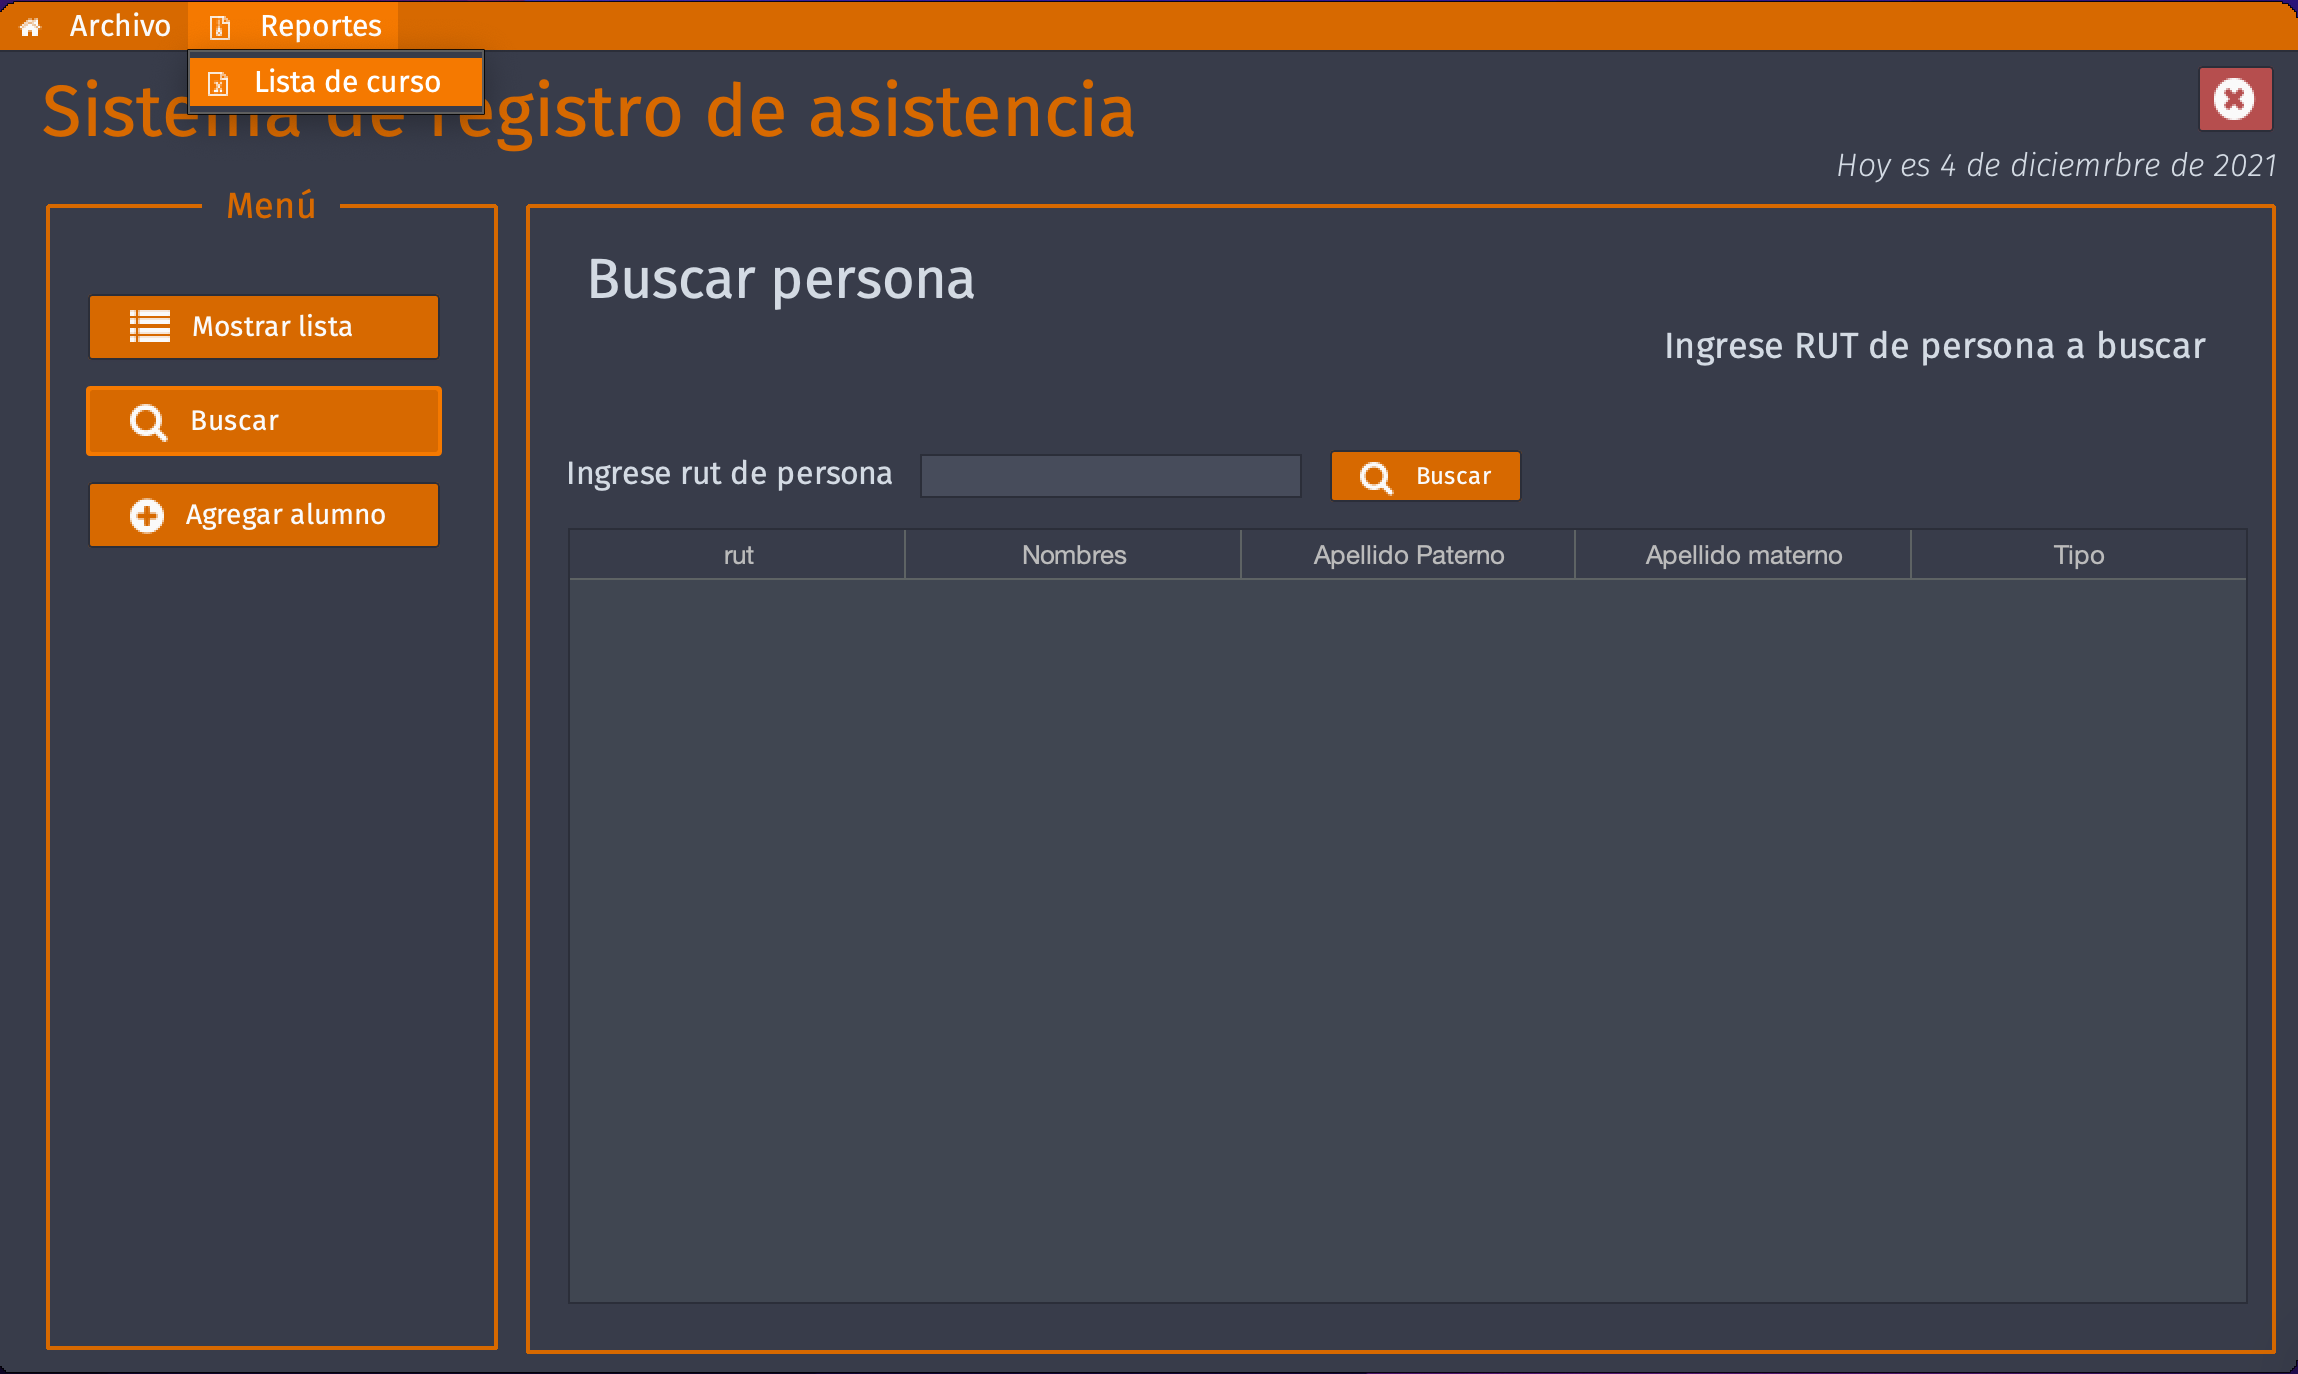
\includegraphics[width=0.7\textwidth]{contents/img/gui/img14}
    \caption{Ventana para buscar persona}
    \label{fig:gui14}
\end{figure}

\clearpage

\textbf{Confirmación para salir de la aplicación}

\begin{multicols}{2}
    \darkBox{Confirmación: Modo oscuro}{
        \centering
        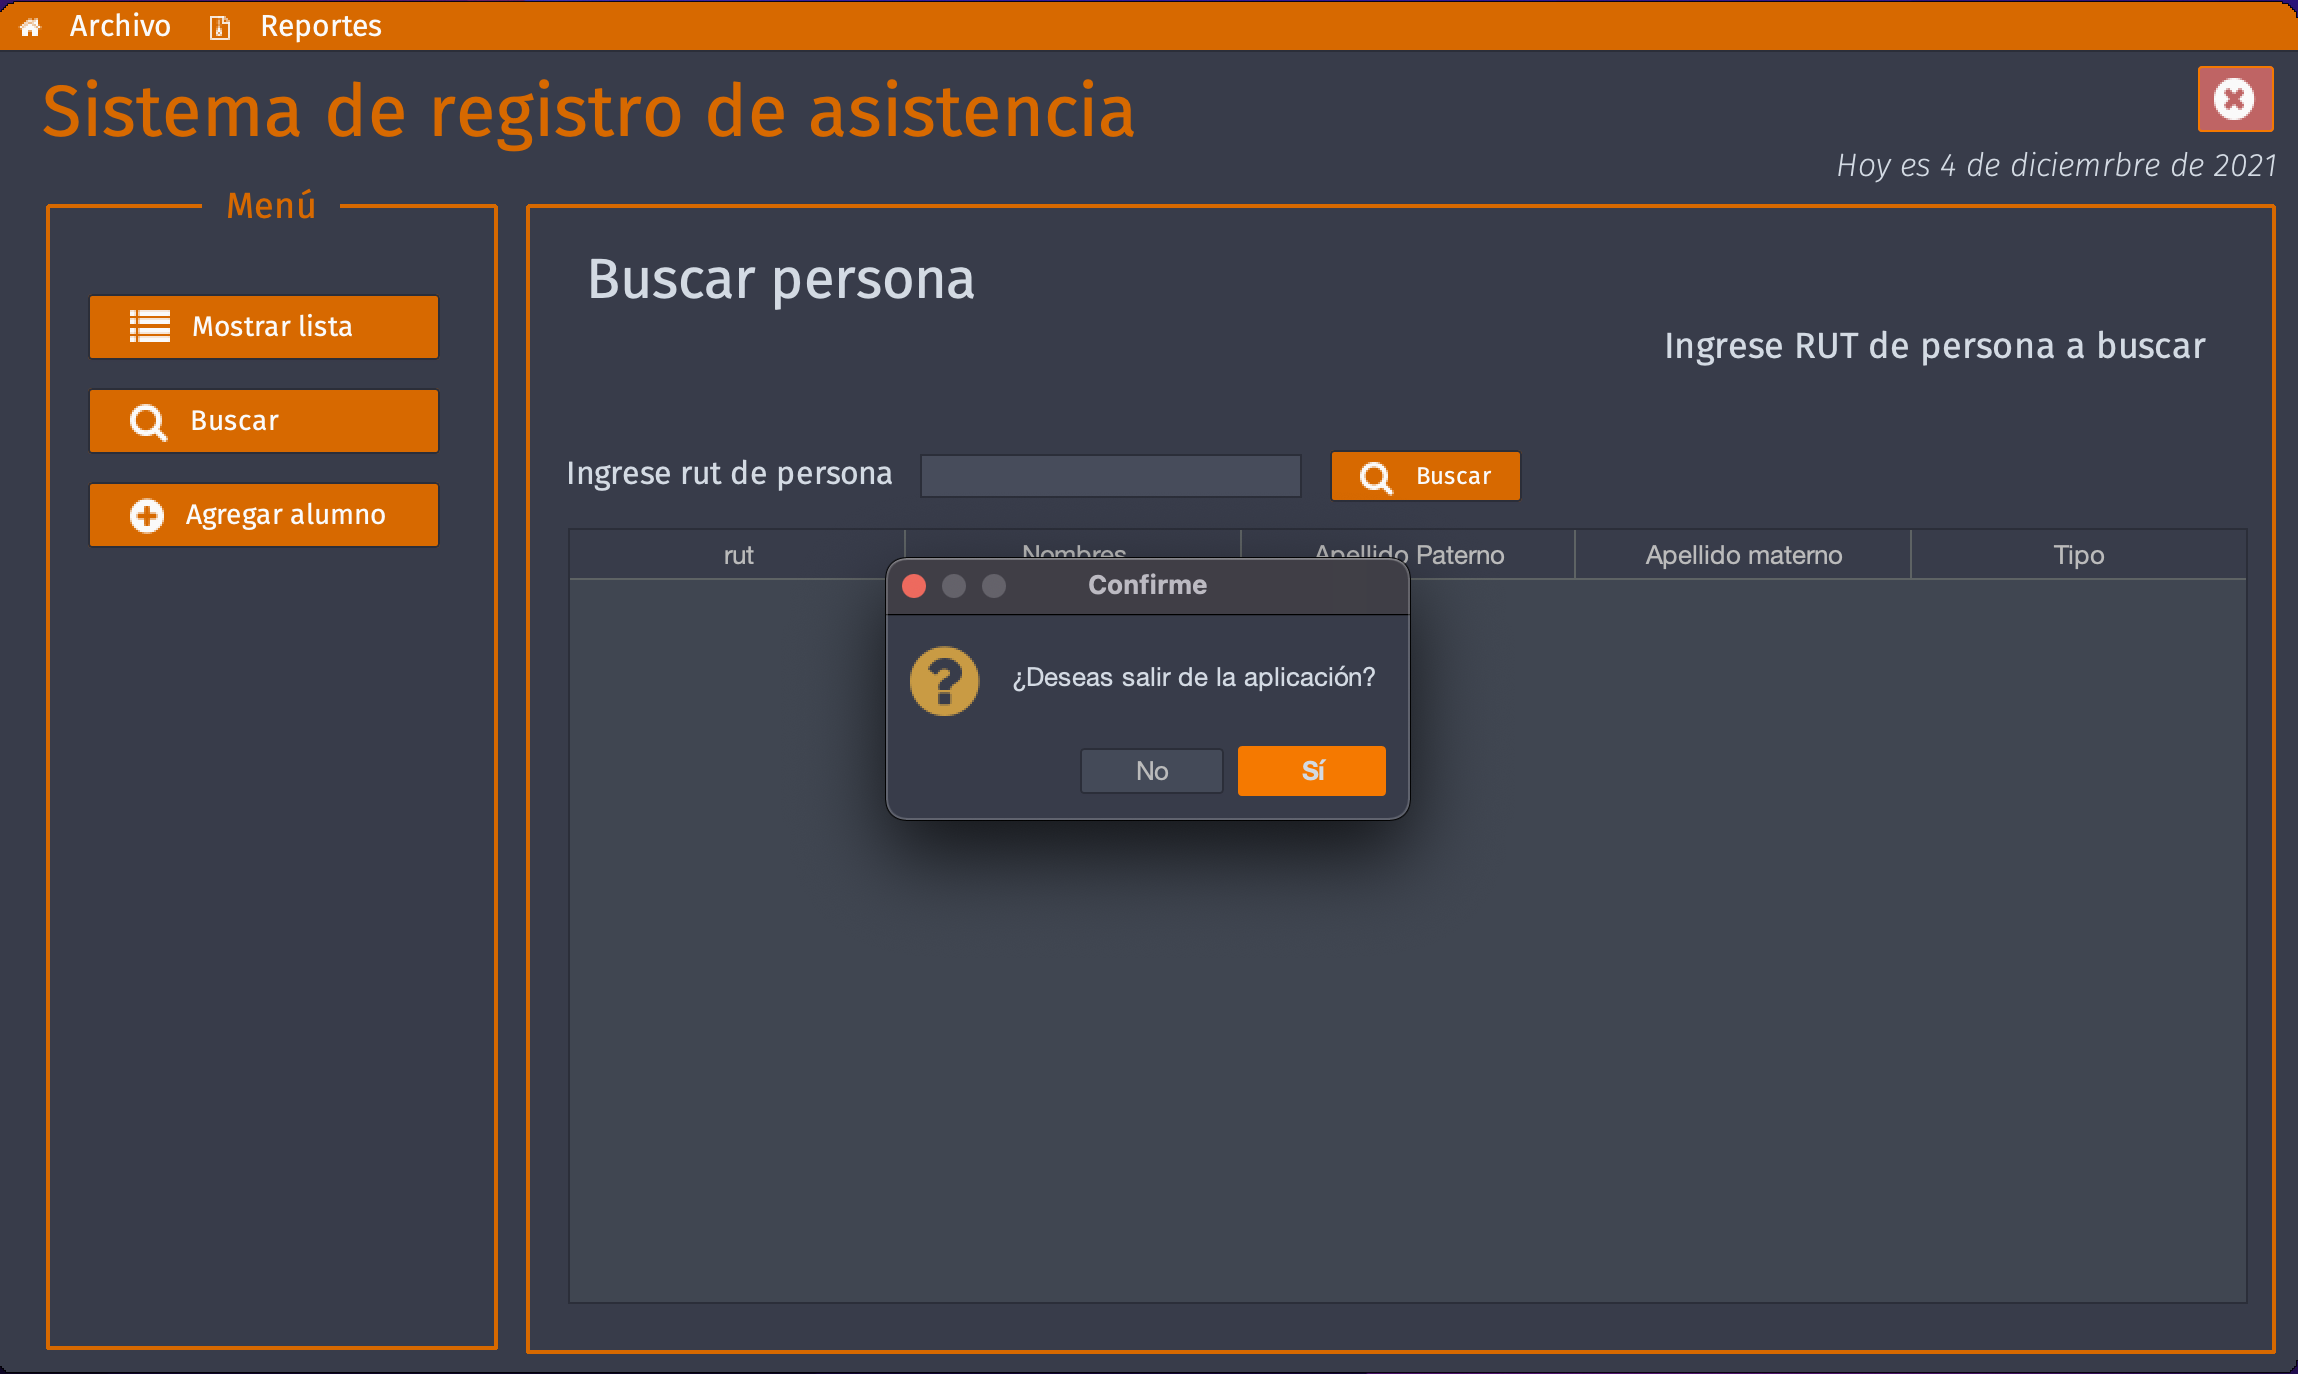
\includegraphics[width=1\textwidth]{contents/img/gui/img18}
        \label{fig:gui18}
    }

    \columnbreak

    \darkBox{Confirmación: Modo claro}{
        \centering
        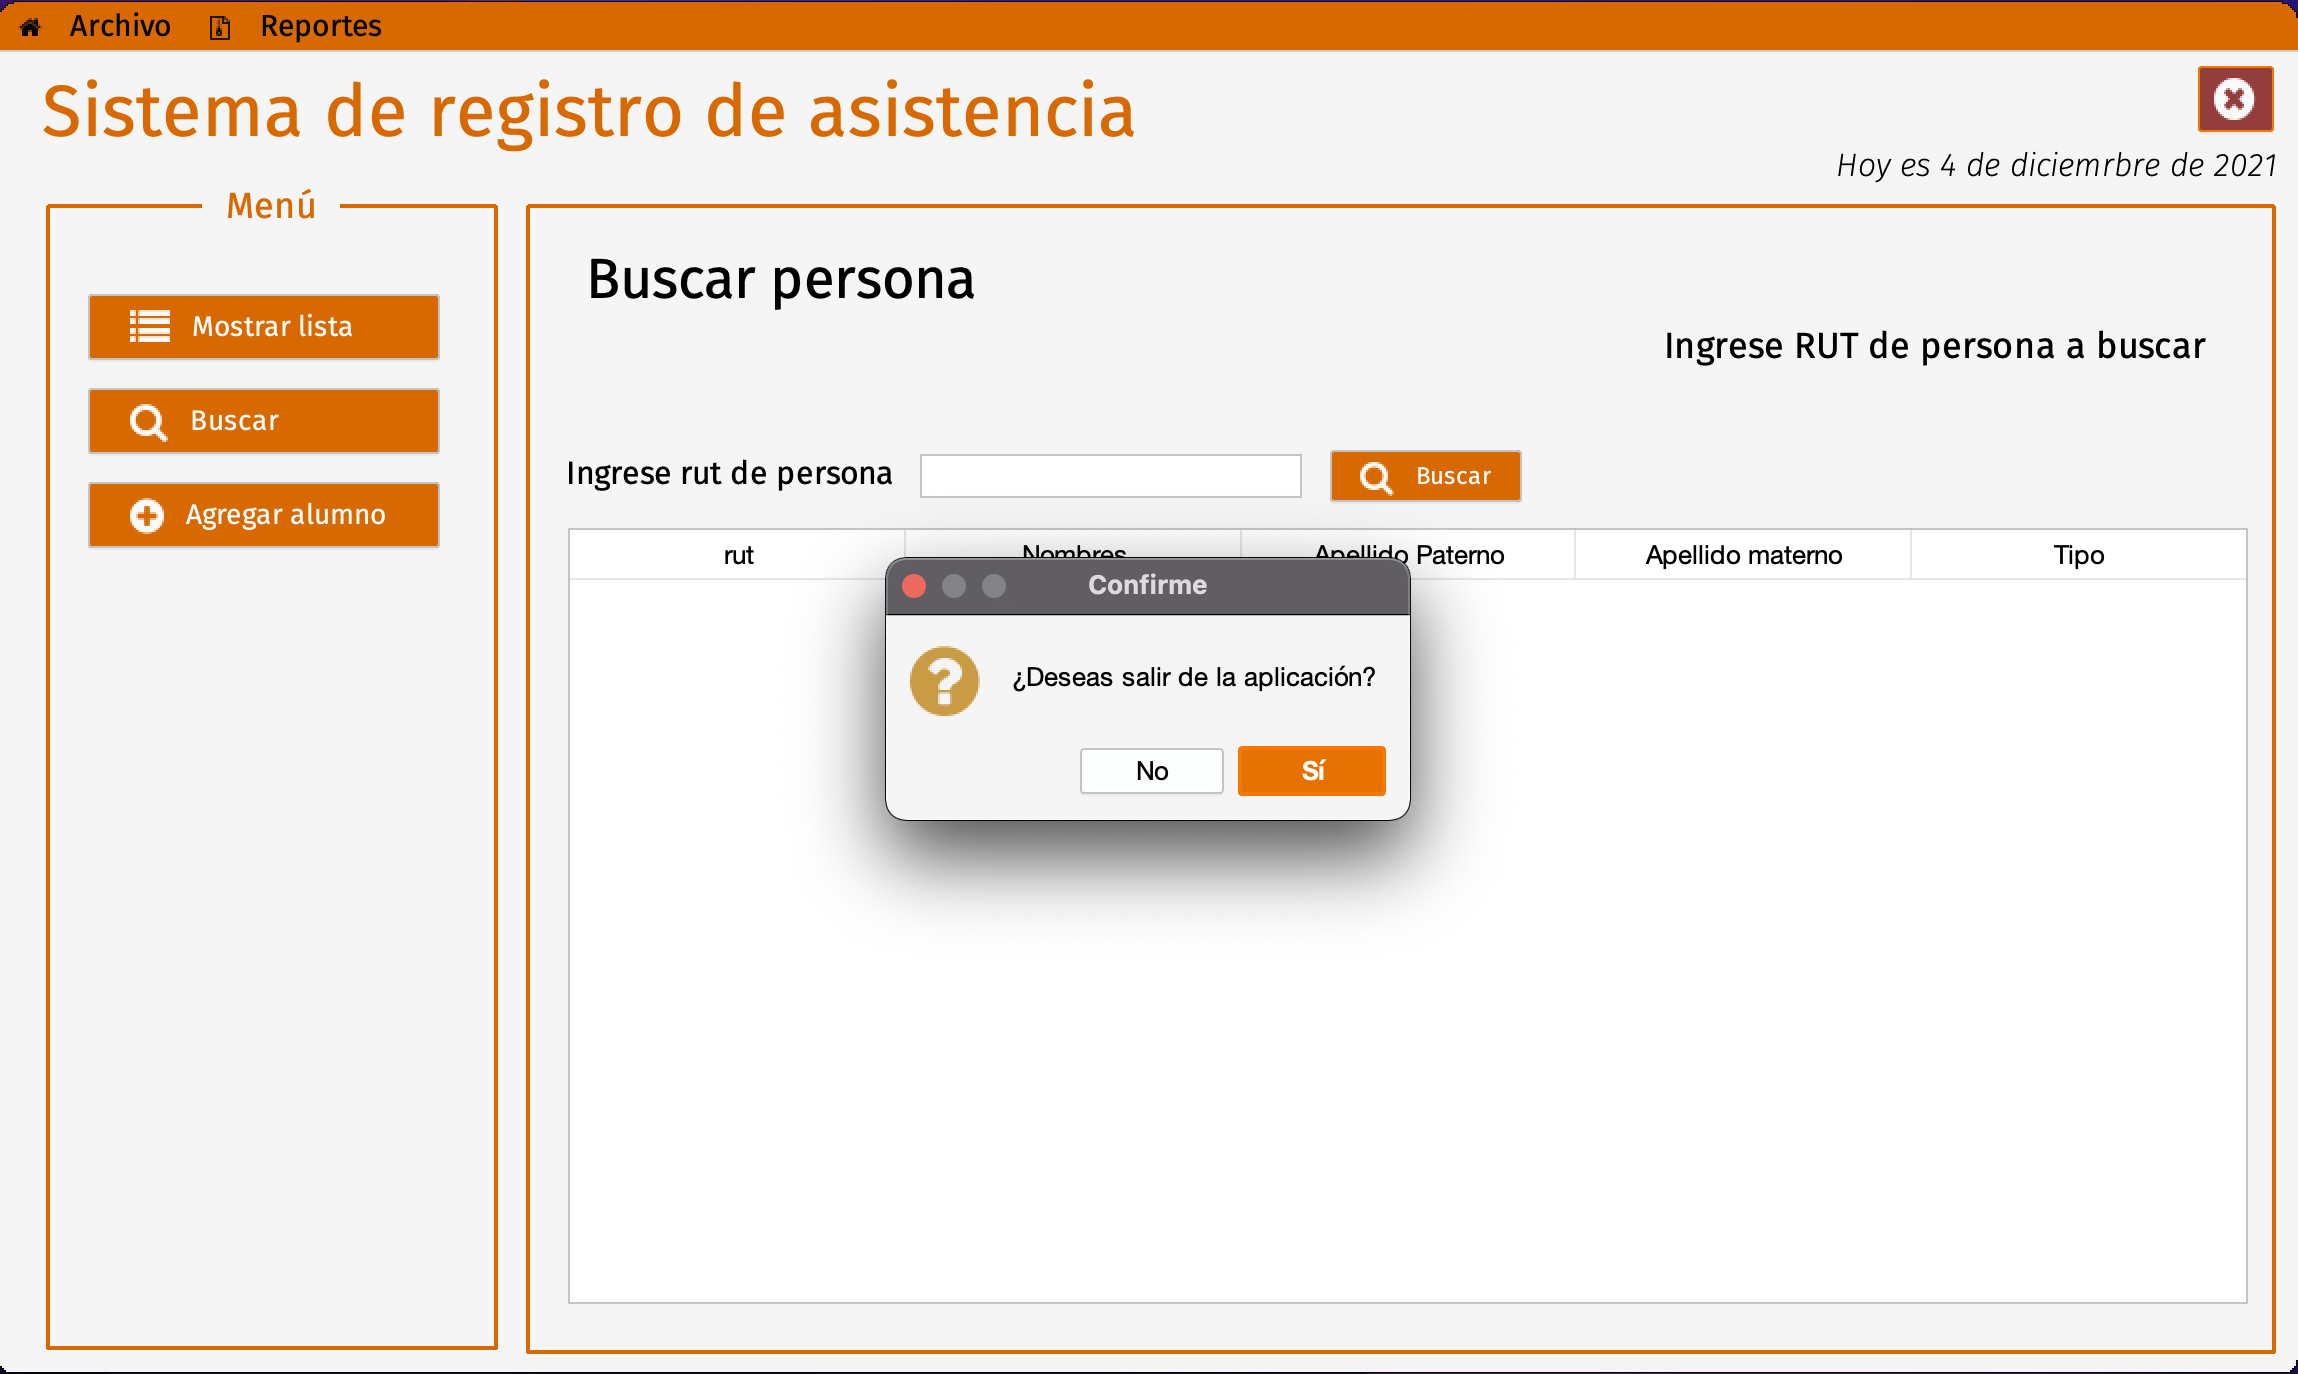
\includegraphics[width=1\textwidth]{contents/img/gui/img19}
        \label{fig:gui9}
    }
\end{multicols}

\subsection{Se debe aplicar encapsulamiento y principios OO}

Lorem ipsum dolor sit amet, consectetur adipiscing elit. Donec et sem luctus, finibus mauris eget, euismod arcu. Morbi at mollis risus. Praesent consequat justo tellus, ac pretium urna lacinia quis. Ut sagittis cursus finibus. Morbi pellentesque vulputate tincidunt. Aliquam at pretium tellus, et vehicula velit. Nunc turpis metus, porttitor sit amet aliquam ut, venenatis quis elit. Nam tincidunt venenatis tortor, ac sodales libero varius nec. Donec vestibulum leo a metus rutrum, vitae elementum diam suscipit. Quisque non mauris rutrum, lacinia lectus id, viverra dui. In leo quam, ultrices vitae suscipit quis, porttitor quis turpis. Vestibulum semper ligula sit amet diam scelerisque gravida.

\subsection{Continuidad en la utilización de GitHub (Realización de al menos 3 Commit adicionales a los ya hechos en la parte A)}

Lorem ipsum dolor sit amet, consectetur adipiscing elit. Donec et sem luctus, finibus mauris eget, euismod arcu. Morbi at mollis risus. Praesent consequat justo tellus, ac pretium urna lacinia quis. Ut sagittis cursus finibus. Morbi pellentesque vulputate tincidunt. Aliquam at pretium tellus, et vehicula velit. Nunc turpis metus, porttitor sit amet aliquam ut, venenatis quis elit. Nam tincidunt venenatis tortor, ac sodales libero varius nec. Donec vestibulum leo a metus rutrum, vitae elementum diam suscipit. Quisque non mauris rutrum, lacinia lectus id, viverra dui. In leo quam, ultrices vitae suscipit quis, porttitor quis turpis. Vestibulum semper ligula sit amet diam scelerisque gravida.
